\documentclass[tikz]{standalone}
\usepackage{pgfplots}
\pgfplotsset{compat=1.15}
\usepackage{mathrsfs}
\usetikzlibrary{arrows,calc}
\usepackage{tkz-euclide}

\usepackage{fp}
\pagestyle{empty}

\definecolor{AngleClr}{rgb}{0,0.39215686274509803,0}
\definecolor{ShapeClr}{rgb}{0.6,0.2,0}

\begin{document}

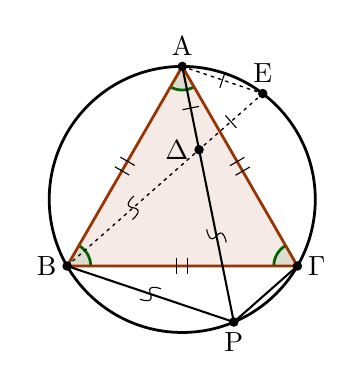
\begin{tikzpicture}[scale=.75]
\tkzSetUpLine[line width=1pt,color=black]
\tkzSetUpPoint[fill=black]

\tkzDefPoints{0/0/B,1.95/3.38/A,3.9/0/C,2.6325/0/Z}

\tkzDefTriangleCenter[circum](A,B,C)
\tkzGetPoint{O}
\tkzDrawCircle[black,line width=1.0pt](O,A)

\tkzInterLC(A,Z)(O,A) \tkzGetPoints{P}{a}
\tkzInterLC(A,P)(B,P) \tkzGetPoints{b}{D}
\tkzInterLC(B,D)(O,A) \tkzGetPoints{E}{c}

\tkzFillPolygon[fill=ShapeClr,fill opacity=0.1](A,B,C)

\tkzFillAngles[fill=AngleClr,size=.4,fill opacity=0.1](C,B,A A,C,B B,A,C)
\tkzMarkAngles[line width=1pt,size=.4,color=AngleClr](C,B,A A,C,B B,A,C)

\tkzDrawPolygon[color=ShapeClr](A,B,C)
\tkzDrawPoints[size=3](A,B,C,P,E,D)
\tkzLabelPoint[above](A){$\rm A$}
\tkzLabelPoint[left](B){$\rm B$}
\tkzLabelPoint[right](C){$\rm \Gamma$}
\tkzLabelPoint[below](P){$\rm P$}
\tkzLabelPoint[above](E){$\rm E$}
\tkzLabelPoint[left](D){$\rm \Delta$}


\tkzDrawSegments[line width=0.75pt](A,P B,P C,P)
\tkzDrawSegments[line width=0.5pt,color=black,dashed,dash pattern=on 1pt off 1.75pt](B,E A,E)

\tkzMarkSegments[mark=||,size=3](A,B B,C C,A)
\tkzMarkSegments[mark=s,size=3](P,D D,B B,P)
\tkzMarkSegments[mark=|,size=3](A,D A,E E,D)

\end{tikzpicture}

\end{document}
